\documentclass[pageno]{jpaper}

%replace XXX with the submission number you are given from the ISCA submission site.
\newcommand{\iscasubmissionnumber}{XXX}

\usepackage[normalem]{ulem}
\usepackage[nocompress]{cite}
\usepackage{epsfig}
\usepackage{graphicx}
\usepackage{epstopdf}
\usepackage{ragged2e}
\usepackage{hyperref}
%\usepackage{amssym}
\usepackage{amsmath}
\usepackage{algorithm}
\usepackage{algpseudocode}
\usepackage{listings}
\usepackage{courier}

\begin{document}

\title{
Basic-block Architecture}

\date{}
\maketitle

%\thispagestyle{empty}

%%%%%%% ABSTRACT %%%%%%%
\begin{abstract}

The main factors contributing to the bulk of energy consumption in modern
out-of-order processors are the speculative logic units, dynamic instruction
scheduling modules, and on-chip data movement.  This work reduces
these energy overheads via introducing compiler-generated techniques that enable
near in-order energy consumption while maintaining near out-of-order computation
performance. Specifically, we introduce the notion of coarse-grain program
execution; in this model, program basic-blocks are speculatively run
out-of-order while instructions within each basic-block run in-order.
Basic-block execution closes up to XX\% of the energy gap and XX\% of the
performance gap between in-order and out-of-order.

\end{abstract}

%%%%%%% BODY %%%%%%%
\section{Introduction} 
\label{sec:intro}

As described by~\cite{mcfarlin2013discerning}, the exceptionally high
performance of out-of-order (OoO) processors is fundamentally due to two key
attributes: dynamism and speculation.  Lack of either feature can significantly
impact its performance. 

The key sources of energy consumption in OoO processors is data-movement and __
(back this up).

BBS is a hardware-software scheduling hybrid technique that enables significant
energy savings in the processor while maintaining near the same level of
performance as the out-of-order processor. This hybrid model is constructed
based on the notion of coarse-grain out-of-order execution where the term
coarse-grain refers to the ability of the processor to execute groups of
instructions out of program order. Each group executes its instructions in order
while multiple such groups execute their instructions out of program order.

\section{Related Work}
\label{sec:rel_work}
In this section, we discuss the related work to Basic-block execution (BBE).

Braid~\cite{braid} focuses on static partitioning of instructions into based on
the program data-flow graph to construct instruction clusters called Braids.
Each braid runs as an independent cluster similar to how BBE dispatches
instructions. BBE follows the same line of design methodology with the focus on
evaluating energy saving opportunities of coarse-grain out-of-order scheduling.
The static instruction scheduler schedules each basic-block as whole rather than
fragmenting it into smaller pieces with the goal of minimizing dynamic bulk
scheduling.

Multiscalar~\cite{multiscalar} evaluates a multi-processing units capable of
steering coarse grain code segments that are potentially larger than a
basic-block to its functional units for computation. It uses replaced register
files in each stage to enable communicating all live registers between two
computation units. Multiscalar can be computation units are configurable to be
OoO or InO. BBE solves the same line of problem through a much more energy
efficient design.

Complexity Effective~\cite{complexity} proposes a distributed instruction
window that simplifies the wake-up logic, issue window, and the forwarding logic
design. Unlike BBE, instruction scheduling / steering in Complexity Effective is
done at instruction granularity.

ILDP~\cite{ildp} proposes a architecture for distributed processing that
consists of a hierarchical register file built for communication short lived
registers locally and long lived registers globally similar to BBE. ILDP,
          however, focuses on proposing design building blocks for
          constructing distributed processing architectures. BBE utilizes this
          design methodology to evaluate energy efficiency gains of coarse-grain
          execution.

WiDGET~\cite{widget} is a power proportional grid execution design consisting of
decoupled thread context management and a large set of simple execution units.
It has a static instruction steering protocol to effectively perform instruction
scheduling at runtime.  WiDGET is an extension of teh work by Salverda and
Zilles's\cite{fundamental} work on designing an instruction scheduling cost
model. BBE is a bulk code scheduling solution allowing new energy saving
opportunities.


TRIPS / EDGE~\cite{edge}~\cite{trips} is a high-performance, grid-processing
architecture that uses pure static instruction scheduling using hyperblocks to
map instructions to the grid of computational units. Its primary focus is
improving extracting ILP, TLP and DLP from the program rather than saving energy
efficiency. Hyperblocks use branch predication to group basic-blocks that are
connected connected together through weakly biased branches. While effective for
improving instruction parallelism, hyperblock codes lead to energy inefficient
mis-speculation recovery events that are not suitable for energy aware
technologies.

CLP~\cite{clp} addresses the processor power efficiency concern through a
configurable clustering of simple execution units to build variable-issue
computing units to exploit both thread-level parallelism and instruction level
parallelism. Core Fusion~\cite{corefusion} has a similar design mentality,
    proposing a configurable chip multiprocessor (CMP) architecture. BBE focuses
    on designing an energy efficient and complexity effective single-threaded
    processor.

iCFP~\cite{icfp} is a variant of the CFP~\cite{cfp} design for in-order
processors. It addresses the head-of-queue blocking problem in the InO processor
by building an architecture that, on every cache miss, checkpoints the program
context, steers miss-dependent instructions to a side buffer enabling
miss-independent instruction to make forward progress. CFP enables the use of
small register file and instruction window while keeping the while maintaining
the same level of performance as conventional OoO processors.  BOLT~\cite{bolt}
is a high ILP, high MLP, latency-tolerant (LT) architecture design for energy
efficient out-of-order execution. It uses a slice buffer design that utilizes a
minimal hardware resources. Unlike BBE, iCFP, CFP, and BOLT perform lightweight
{\it{dynamic}} instruction scheduling to manage available instructions and hide
LLC cache misses.

Outrider~\cite{outrider} is a high-throughput architecture that decouples a
single thread context into two parallel {\it{strands}} one for memory and
another for other operations in order to allow LLC miss latency hiding by
helping miss-independent instructions fast-forward through the execution
pipeline. Its goal is to eliminate the herd-to-scale processor structures such
as the instruction window and the OoO scheduling model. BBE is a single-threaded
design focused on hiding LLC latency miss through issuing instructions form
multiple energy efficient BB Window FIFO buffers.

Trace Processors~\cite{trace} propose a similar register hierarchy and
instruction flow design based on dynamic trace processing in the frontend. BBE
is an energy efficient solution focused on offloading majority of instruction
scheduling work to the compiler.

MorphCore~\cite{morphcore} is an in-order, out-of-order processor hybrid
designed to improve single-threaded energy efficiency. It uses {\{it{dynamic}}
instruction scheduling and core-type detection. It achieves 22\% improvement in
energy-delay product while BBE achieves 25\%.

Sun ROCK~\cite{rock} is a dynamic chip multithreading processor with support for
efficient program checkpointing. It is an out-of-order with dynamic instruction
scheduling.

\section{Energy Overheads of OoO}
\label{sec:o3_overhead}

iWindow: update and ready are CAM lookups. both take up a lot of energy

Register Renamer: renaming for short lived registers: lots of table lookups,
         large port count

Register file: lots of renaming means lots of PR's and lots of ports

BPU: lookup per fetch-width is excessive and hence prone to energy loss and
aliasing problems. can only do lookup for H instructions
to reduce port count + traffic of access.

having smaller instructions reduces the decoding overhead making the instruction
decoding energy much smaller.

Squash drain overhead. This process involves either draining the entire ROB upto
the point of flush or define tables that checkpoint program state. The latter
approach is significantly more high performance, esp. for deep pipeline
structures while being more energy consuming for keeping track of program state.
WE choose to evalaute our work against the case with only ROB. 

Squash support in this model eliminates the need for a register rename commit
RAT only because on a squash the younger basicblocks can invalidate the faulty
entries (talk about it the solution later and give a teaser here)

LSQ: fewer mis-speculations because clos-by LS's can't conflict

Pipeline stage resduction: faster BP, fast and fewer RR, faster scheduling

forwarding: arbitrary in OOO, but here it is scheduled to leverage it.


fetch overhead is completely justified because each instruction in this ISA is
shortened, making more than enough room to fetch additional instructions (i.e.
        H).
 

\section{Coarse-grain OoO Execution}
\label{sec:course_grain}

In this work, we introduce the notion of coarse-grain execution where every
cluster of instructions is a unit of execution that is statically scheduled to
run optimally without further dynamic scheduling by the hardware. We call it the
{\it{Phraseblock}}. Phraseblock differs from other instruction clustering
definitions such as superblocks~\cite{superblock} and
hyperblocks~\cite{hyperblock} in that its purpose is to group the set of
instructions that, ideally, can execute without an unpredictable latency
interruption. 

The simplest form of a phraseblock is the program basic-block whose energy and
performance are evaluated in this work. Similar to an instruction, the
basic-block is a single-entry, single-exit unit without any control stalls.
Memory stalls are possible within a basic-block, but with effective static
scheduling, their impact on stalling other independent instructions in the
basic-block is minimized.

\begin{figure}
	\centering
	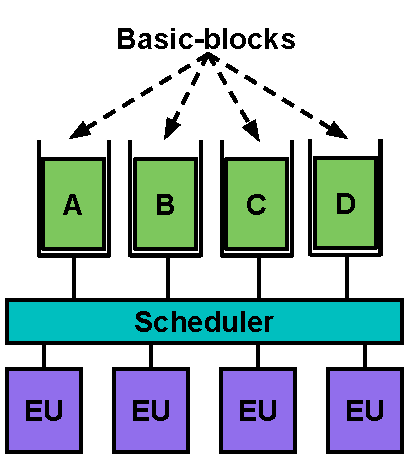
\includegraphics[width=0.5\columnwidth]{fig/coarse_grain_sch.pdf} 
	\caption{Coarse-grain execution model}
	\label{fig:coarse_grain_sch}
\end{figure}

In the presence of unpredictable memory and control stalls, a fully static
schedule cannot deliver the same code quality as a dynamic scheduler like the
Tomosulo's algorithm~\cite{tomasulo}. To address the problem with unpredictable
long latency operations, we propose a new approach in combining static and
dynamic scheduling that leverages the ability of static scheduling in saving
energy while delivering optimal code schedules for parts of the code that need
dynamic scheduling and to leverage the ability of dynamic scheduling in hiding
the latency of unpredictable long latency events such as cache misses. To do so,
    we allow multiple speculative basic-blocks to be in-flight at the same time
    to dynamically contend for resources.  Each basic-block is statically
    scheduled and issues its instructions in-order.  As a result, when a load
    operation in a basic-block misses in the L1, it stalls but other in-flight
    basic-blocks issue instructions to hide its latency.
    Figure~\ref{fig:coarse_grain_sch} illustrates four basic-blocks placed in
    four first-in-first-out (FIFO) instruction queues, contending to schedule
    their instructions on one of the available execution units (EU).

\section{Code Generation}
\label{sec:code_gen}

In this section, we discuss the compiler passes used to construct BBE program
binary as well as the micro-architectural blocks designed to support BBE.

We run binary translation on the x86 ISA to generate the program control flow.
Once basic-blocks are identified, a number of elements in each BB must be set;
special basic-block header (\texttt{Head}) instructions must be inserted, an
energy-aware register allocation model is run, and instruction scheduling is
done to generate the optimal static schedule for each basic-block.  In this
work, a basic-block is defined to end with a \texttt{br}, \texttt{jmp},
    \texttt{call}, or \texttt{return}. It is also terminated when the the
    basic-block reaches 16 instructions. %TODO specify how rare is this

\begin{figure}
	\centering
	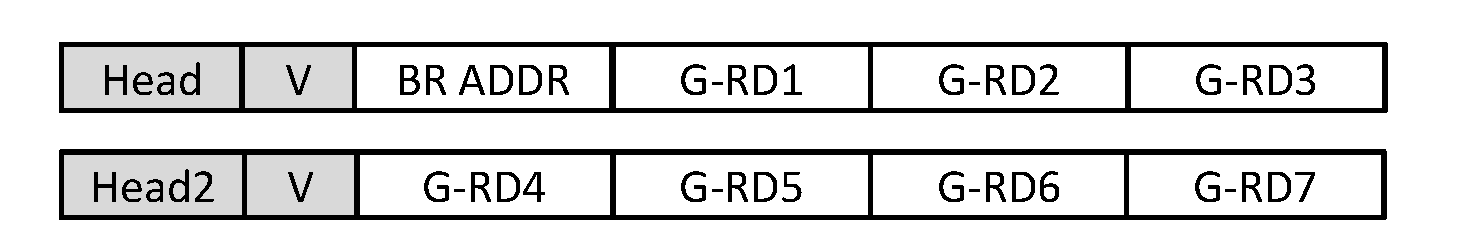
\includegraphics[width=1.0\columnwidth]{fig/header_ins.pdf} 
    \caption{\texttt{Head} and \texttt{Head2} instructions represent BB
        header information. \texttt{Head2} is only used for basic-blocks with
            more than three global read operands. BR ADDR represents the address
            offset of the branch operation at the end of the BB. V bits specify
            how many of the register operands are valid and whether BR ADDR
            holds a valid entry.}
	\label{fig:header_ins}
\end{figure}

Two register allocation passes are done on the compiler to generate instruction
operands. The first pass finds the register operands live beyond the boundaries
of the basic-block, and the second pass allocates registers live only within the
basic-block boundaries. The former is a global register and the latter is a
local register. The motivation to build separate register operands is to avoid
register renaming on short-lived registers and instead store them in statically
managed, small and energy efficient register files. As discussed later, we find
the energy difference between accessing a physical register file and a local
register to be about 14x. To further save energy, for cases with a global DEF
followed by one or more global USE of the same physical register, a copy of the
operand is stored locally for the USE operation(s). When more then one operand
in a basic-block reads from a global register, a \texttt{MOV loc, glb}
operation is inserted prior to the reads to bring the operation to the local
register space prior to the readers. With these assumptions, global read and
write operands within each basic-block access the global register file once.

At runtime, the decoder stage identifies the beginning of a new basic-block by
the special {\it{Header}} instruction. As shown in Figure~\ref{fig:header_ins}
Header contains 1) the instruction address of the branch instruction in the BB
(if any) and 2) the global ready architectural register read operands. BR ADDR
is used to lookup the BPU to find the next basic-block. It is stored in Header
to 1) initiate fetch of the next speculative BB early, and 2) to enable BPU
access {\it{after}} instruction decode, when Head is detected, but branch is
potentially not yet fetched so that {\it{only}} Head instructions access BPU
rather than all fetched instructions. Read register operands are removed from
their original operands and compressed into Head to 1) enable renaming bypass by
all instructions except Head, and 2) shorten the frontend pipeline depth.
\texttt{Head2} is an extension to \texttt{Head} for BB's with more than three
global operands. %TODO how often?

%TODO discuss instruction scheduling


\section{Microarchitecture}
\label{sec:arch}

Coarse grain execution exposes energy saving opportunities in most pipeline
stages. In this section we discuss the flow of basicblocks through different
pipeline stages and elaborate on how energy is saved in each stage.

Below, we discuss the various architectural components of this architecture.
Figure XX illustrates the processor stages in detail.

\subsection{Basicblock Structure}
\label{sec:bb_struct}

What: discuss bb binary structure including its header contents: branch address.
Also explain the hardware support structure to hold register renamed values for
each global operands (both rad and write). it also contains the BB SN.

Why: to show how we save energy by BP lookup and energy efficient renaming
(renaming buffer is tiny, and cheap to access for both ready-check and wake-up
 logic). energy efficient and more high performance branch prediction.

(make a note that bb header for holding register operands is a CAM array)

% Basicblock boundaries are explicitly annotated by the compiler in the program
% binary through special header instructions (H) that contain certain key
% information about the BB; H instructions hold the BB branch instruction address
% (unless the BB is terminated without a branch or jump operation), global read
% registers, and global write registers used in the BB. Figure XX illustrates the
% organization of each H instruction.
% 
% Contrary to existing processors where the branch-prediction unit (BPU) is looked
% up on every fetch group regardless of the type of instructions in the fetch
% group, BB looks up the branch predictor only through H instructions. Immediately
% after the decode stage, H instructions feed the address of the upcoming branch
% instruction to BPU to find the PC of the next basicblock. This approach
% significantly reduces the traffic to BPU reducing mis-predictions due to
% aliasing and lookup energy consumed unnecessarily by non-branch instructions.
% 
% Global write registers used by instructions in the basicblock are incorporated
% in H so that ?.
% 
% Global read registers used by instructions in the basicblock are incorporated
% in H so that the wake-up logic would simply ?.
% 
% Discussion on instruction overhead (for i-cache) of adding H instructions to the ISA.

\subsection{CPU Frontend}
\label{sec:cpu_frontend}

discussion of register renaming and branch prediction lookup and update models.

% The processor frontend consists of the branch-prediction, fetch, decode, and
% register rename stages. Branch prediction only looks up H instructions. Fetch
% and decode stages are designed similar to existing architectures with
% configurable withs of 2, 4, 8. Contrary to the OoO model where register renaming
% happens in dispatch stage, here register renaming is done right after decode
% (explain why).  The register rename unit is only accessed by H instructions.
% Local registers do not access the register rename unit.
% 
% Given the smaller utility of register renaming, this processor can use a
% smaller set of physical registers (less area and energy per access).

\subsection{CPU Backend}
\label{sec:cpu_backend}

The backend consists of several basicblock window buffers used to store
basicblock operations and the meta-data associated with each BB, local registers
for each basicblock, a global register file, execution units, basicblock reorder
buffer (BBROB), a load-store queue model, and the wake-up logic.

%\subsubsection{Basicblock Window}
\label{sec:bb_window}

\textbf{BB Windows} are FIFO buffers used to store up to 16 outstanding
instructions.  Instructions in a BB Window execute in-order. In
Figure~\ref{fig:bb_arch}, eight BB Windows are shown where each BB Window can
issue up to two instructions per cycle. Each cycle, the head of each BB Window
is checked for ready instruction(s). If more than four instructions are
available, the four oldest instructions are issued. Since BB Windows are FIFO
structures, we find their lookup and update energy overhead is an order of
magnitude smaller than reservation station tables.
%justify hwy two instructions

\begin{figure}
	\centering
	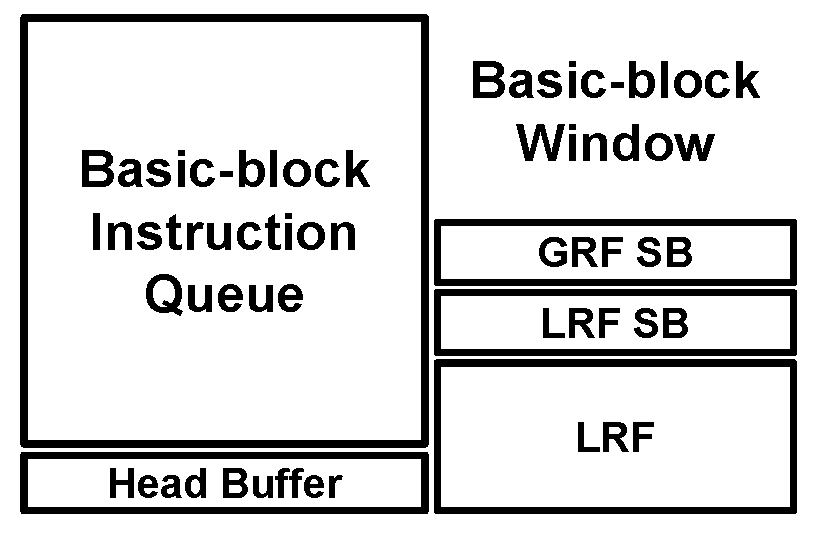
\includegraphics[width=0.6\columnwidth]{fig/bb_window.pdf} 
	\caption{Basicblock window structure}
	\label{fig:bb_window}
\end{figure}

\textbf{LRF} is a simple register file with at most 8 statically
allocated register elements. Each BB Window has its own dedicated basic-block
that is used to support storing register entries that are live only within the
basic-block lifetime. Once the basic-block completes its execution, the content
of these LRF's are invalidated. Figure~\ref{fig:bb_window} illustrates the hardware
elements supporting BB Window. GRF SB and LRF SB are the scoreboard tables used
to store the basic-block global read. A LRF SB entry is made valid once its
corresponding write operands updates the LRF. A GRF SB entry is also updated
when a global operands is about to write its valud to the GRF; the difference is a
global operand broadcasts to all GRF SB's. Since GRF SB's are small CAM arrays
with at most 7 global entries, the energy overhead of updating them is
negligible compared to an instruction window broadcast update.

Head Buffer in Figure~\ref{fig:bb_window} holds the instruction(s) pending to be
issued from the BB Window.

Figure XX shows the average number of in-flight basicblocks for SPEC2006
benchmark.

%Instructions hold offset to the instruction rather than to actual register
%address. This cuts back the register address by half (making the ISA shorter)
%    and also enable RAM lookup to the GRF table upon lookup.

%GRF scoreboard update is CAM baesd, but its lookup is RAM based. (very cheap)
%    update: CAM lookup to address ready bit
%    lookup: RAM lookup to the 1bit entry.



\subsubsection{Register File Structure}
\label{sec:reg_files}

We find that on average roughly 50\% of data communication in SPEC benchmarks
are done across def-uses that have sub-basicblock live ranges. Such registers
do not need to be register renamed if an additional register space is available
for them to temporarily hold their values for the upcoming user instruction.  As
a result, two classes of registers are defined in this architecture: local registers
and a global register. The global register is a big register file with register
renaming support. Local registers, on the other hand, are small register
file blocks with no register renaming; allocation for these registers is
done at compile time.  Global registers are designed for data communication
across basicblocks while local registers are designed for data communication
within a bsaicblock.

\subsubsection{Basicblock Reorder Buffer (BBROB)}
\label{sec:bb_rob}

Contrary to the OoO execution model where the program order is tracked at
instruction granularity through the reorder buffer (ROB), in this design, we only
track program order at basic-block granularity. BBROB is a content addressable
memory array (CAM) with only 16 entries (~10x smaller than ROB size in OoO) that
enables issuing, committing, and squashing basic-blocks as a whole in one cycle
(per basic-block). The smaller size of BBROB compared to a ROB enables
significant energy savings.

BBROB is marked complete when all its operations are completed. Complete
operands increment the completion counter in their BBROB entry. Once the counter
reaches the expected BB size, the BB is marked complete. BBE can commit up to
one BB per cycle, allowing bulk commit using one port to the table. At commit,
    the global write operands in the BB will be marked non-speculative.

%Discussion on what is held on each BBROB entry: BBID, number of completed
%basic-block instructions, total number of instructions in the BB that need to
%complete, valid bit, mis-speculation bit, global physical register writes.

%Discussion on how basic-block entry updates the GRF upon commit through its
%global physical register writes (its GRF write register(s) go from speculative
%to architectural).

%After the decode stage, a BB entry is reserved in BBROB, and when all
%instructions in a basic-block are completed and the basic-block reaches the head
%of the BBROB, the basic-block is committed as a whole in one cycle. Upon a branch
%mis-speculation event (either branch or memory), younger basic-blocks are flushed
%in one cycle. (TODO: talk more about the squash process here)


\subsection{Basicblock Scheduling}
\label{sec:scheduling}

Instruction scheduling example.

Scheduling consists of:

1) ready check: find ready instructions from head of BB - what are the
dependency checks done?

2) update check: blast write operands to all BB-header buffers. 

3) discussion of available bbWindow detection and bbWidnow allocation

% This unit is broken into two main sub-units: instruction issue and instruction
% update. The instruction issue unit looks for ready instructions at the
% head of each basicblock window buffer on every cycle. The instruction udpate
% unit updates global and local register values.
% 
% Update unit discussion goes here. It talks about updating local registers and
% their ready bits, and updating basicblock headers to indicate if the global
% operands of different instructions in a basicblock are ready.
% 
% Issue unit discussion goes here. It talks about how the issue unit checks the
% corresponding local and global operands of an instruction to determine if the
% instruction is ready. Global operands availability is checked by looking up the
% BB header (where the update unit marks a valid bit for each pgysical global
% operand that is ready) and the local operands are checked by lookup
% their up valid bit in the corresponding LRF. 
% 
% Here we also discuss the energy efficiency implications of looking up the head
% of 16 basicblock buffers rather than blasting through a 120 entry instruction
% window (which is a CAM array). We also discuss how basicblock headers help
% reduce the number of check-for-ready-operands accesses to GRF by keeping ready
% information for each global register value in the header of the BB.
% %TODO you need to implement this

\subsection{Squash Handling}
\label{sec:speculation}

In BBE, squash events are handled at basic-block granularity. To avoid wasting
{\it{useful}} instructions executed in a mis-speculated BB, the compiler uses
profiling information to separate weakly biased branches form the rest of the BB
into a single-instruction BB. Less than XX\% of useful instructions are wasted
in BBE.

The average number of BB's squashed per mis-prediction event is 6 where each
basic-block has an average of 3 global write operands. BBE is able to invalidate
register renaming entries within 5 cycles which is comparable to the number of
cycles OoO takes to restore a checkpoint and restart the execution. This
approach eliminates the need for both program checkpointing and a second
register alias table.

% how many cycles does it take to load a checkpoint?
% how much energy is it to track checkpoints?


%Memory mis-prediction is less likely in this model as each basicblock buffer
%runs in-order (no chance of mis-speculation between load-stores within a
%basicblock). We also say that mis-speculation handling is the same for
%both memory and branch.


\section{Simulation Framework}
\label{sec:simulation}

Discussion on the simulator parameters, use of Pintool, pinpoints, wrong-path
execution support, energy model integration.

Discussion on the benchmark

Simulator framework: pin, wrong-path, energy, speculation, function vs. timing
simulation, pin-points?

\section{Results Discussion}
\label{sec:discussion}


Figure~\ref{fig:overall} illustrates the performance, energy, and the
energy-delay (ED) product  of the OoO and BB cores normalized to the InO
processor.  On average, BB closes 70\% of the performance gap between INO and
OoO while closing 66\% of their energy gap. Overall, the energy delay product of
BB is 27\% more effective than InO and 25\% more effective than OoO.
\begin{figure*}[h]
	\centering
	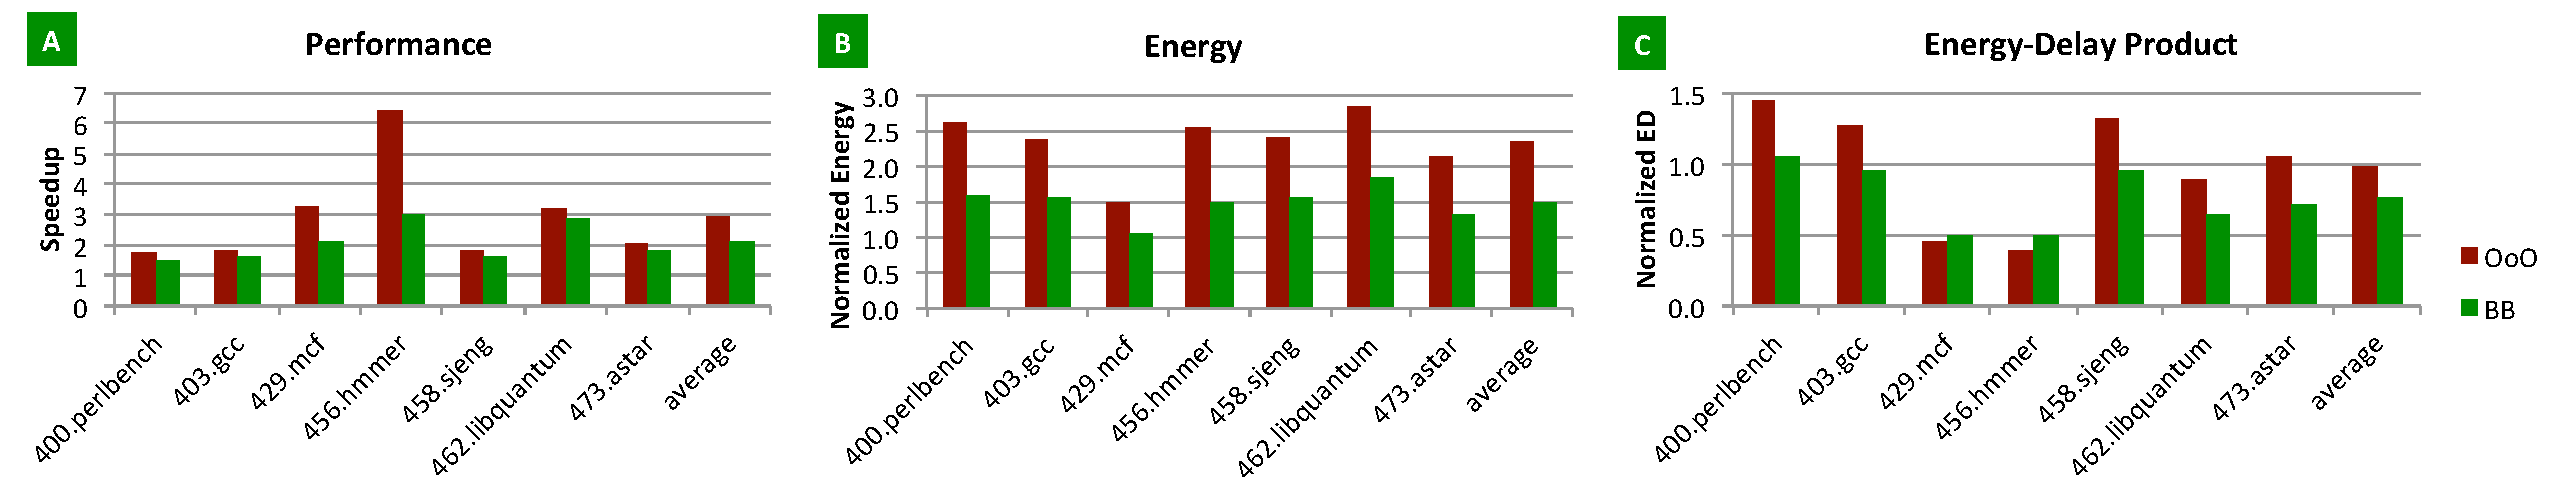
\includegraphics[width=\textwidth]{result/overall_perf.pdf} 
    \caption{(A) $IPC_{CORE}/IPC_{BASE}$, (B) $E_{CORE}/E_{BASE}$, (C)
        $ED_{CORE}/ED_{BASE}$; $CORE$ refers to BB and OoO and $BASE$ refers to
            INO core.}
	\label{fig:overall}
\end{figure*}

Figure~\ref{fig:ep} illustrates the energy versus performance plot for the three
processors when using 2-wide, 4-wide, and 8-wide architectures. Each point on
the figure is the average (speedup, energy) of SPEC benchmarks evaluated here.
While OoO provides best performance, we see the BB architecture with 8
functional units is at the lowest right corner of the graph, making it the best
design choice. Comparing Figure~\ref{fig:ep} with Figure~\ref{fig:insight} shows
the effect of the BB architecture in pushing the trend towards the more energy
efficient corner. There is still more work to be done to push the performance
point of BB further to the right.
\begin{figure}[!htbp]
	\centering
	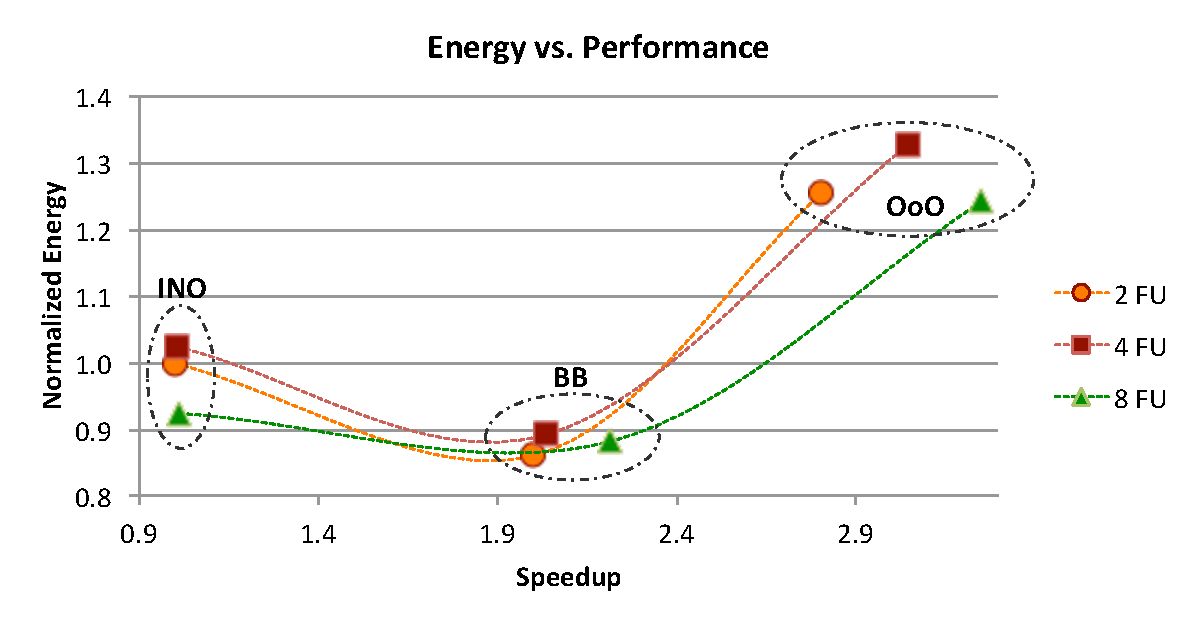
\includegraphics[width=1.0\columnwidth]{result/ep.pdf} 
    \caption{Energy vs. Performance Trend for OoO, BB, \& InO}
	\label{fig:ep}
\end{figure}

Figure~\ref{fig:bbWin_size} illustrates the change in performance and energy of
BB when the BB Window size changes. Recall that the number of available FIFO
slots in these buffers define how the compiler partitions basic-blocks. The
smaller the FIFO size, the more fine grain the code, the more the number of BB's
in-flight to issue instructions. Overall, we observe 15\% average performance
drop and XX\% energy gain when BB Window size changes from 5 to 15 entries.
\begin{figure}[!htbp]
	\centering
	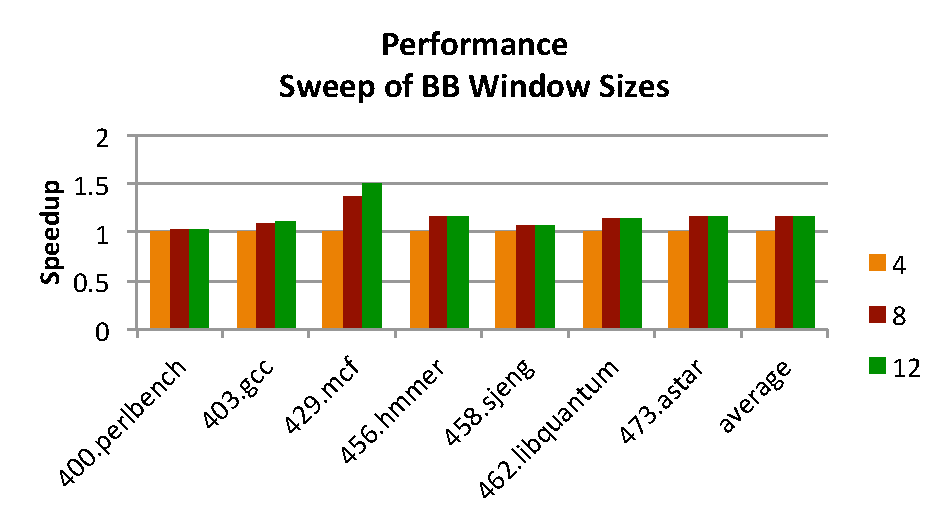
\includegraphics[width=1.0\columnwidth]{result/bbWin_size.pdf} 
    \caption{Performance \& energy change with sweeping the BB Window FIFO queue size}
	\label{fig:bbWin_size}
\end{figure}

Figure~\ref{fig:bbWin_ins_cnt} evaluates the effect of BB Window count on the
performance of BB architectures. We observe 16\% speedup gain between 4 and 8
instruction BB Windows, but not so much beyond. This result suggests  eight BB
Windows are sufficient to get optimum performance gains while keeping the energy
at a relatively low value. Because gcc has small basic-blocks with independent
instructions, it makes best use of the extra BB Window resources to improve the
ILP by up to 50\% while saving up to 8\% in energy as a result.
\begin{figure}[!htbp]
	\centering
	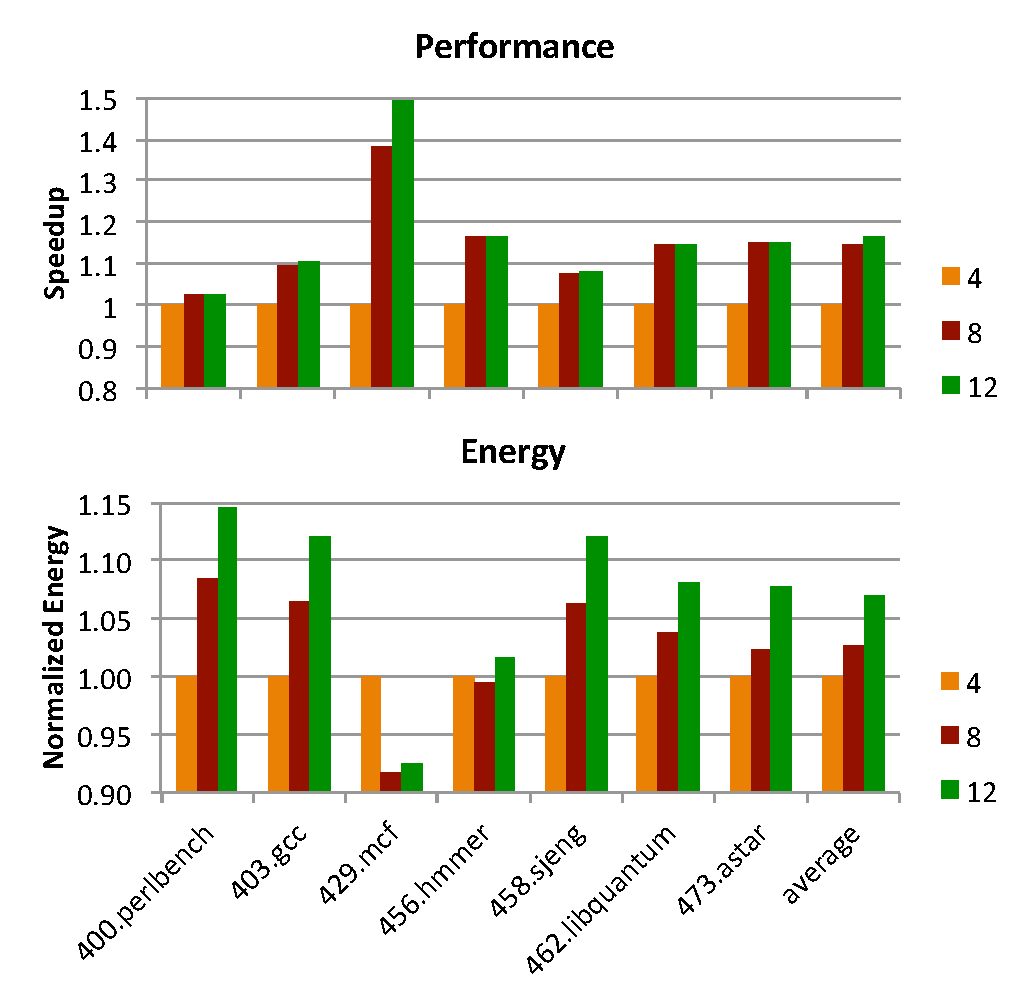
\includegraphics[width=1.0\columnwidth]{result/bbWin_ins_cnt.pdf} 
    \caption{Performance \& energy change with sweeping the number of BB Windows}
	\label{fig:bbWin_ins_cnt}
\end{figure}

Figure~\ref{fig:bbWin_port} evaluates the performance improvement trend as the
number of read ports for BB Windows increase from 1 to 8 ports. While eight
ports provides 11\% average performance gains, three ports provides 10\%.  Given
the XX\% energy overhead of 8-ported BBWindows, we find three read ports the
optimal port count for achieving optimal ED product.
\begin{figure}[!htbp]
	\centering
	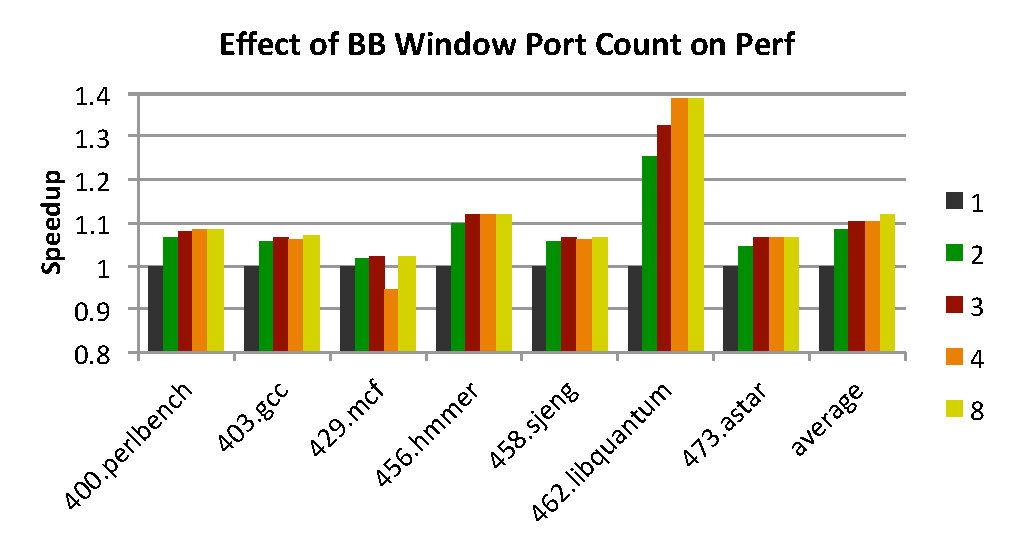
\includegraphics[width=1.0\columnwidth]{result/bbWin_port.pdf} 
    \caption{Performance \& energy change with sweeping the number of BB Window
    ports}
	\label{fig:bbWin_port}
\end{figure}

Figure~\ref{fig:lrf_effect} shows 12\% average increase in speedup and 19\%
reduction in energy consumption of BBE when the register allocator uses LRF
versus when it only uses the global register file for all operations.
\begin{figure}[!htbp]
	\centering
	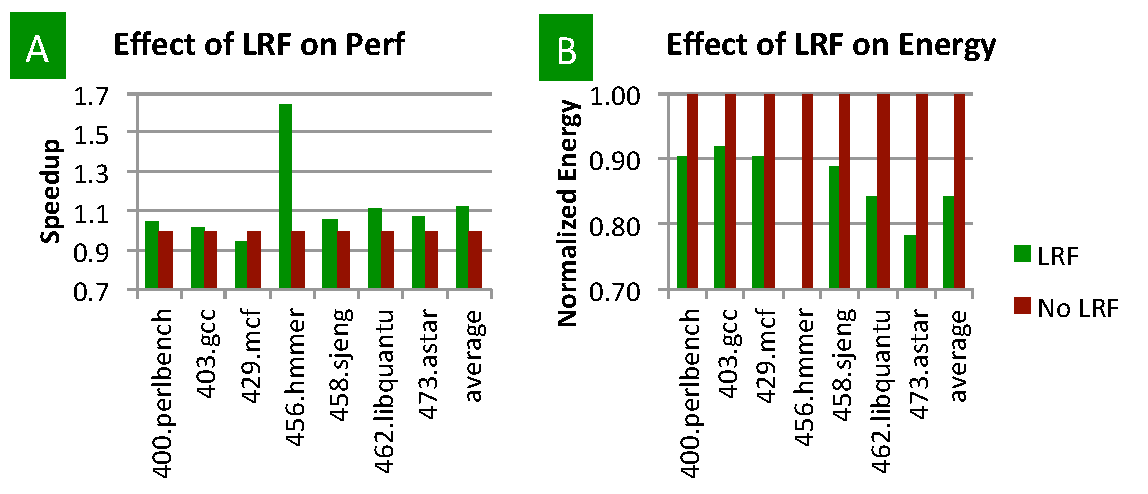
\includegraphics[width=1.0\columnwidth]{result/lrf_effect.pdf} 
    \caption{Performance \& energy change with sweeping the number of BB Windows}
	\label{fig:lrf_effect}
\end{figure}


As mentioned earlier in the paper, BBE benefits from optimal basic-block
instructions scheduling, making each basic-block issue instructions at the
highest issue rate possible. This implies enabling the scheduler to identify
data dependency chains in the code and scheduling instructions such that they
can be issued back-to-back while using the common data-bus for reading their
input operands. Figure~\ref{fig:forwarding} shows BB is 39\% more effective in
leveraging data-forwarding while issuing instructions. The bar charts are
normalize to the forwarding ability of the InO core. 
\begin{figure}[!htbp]
	\centering
	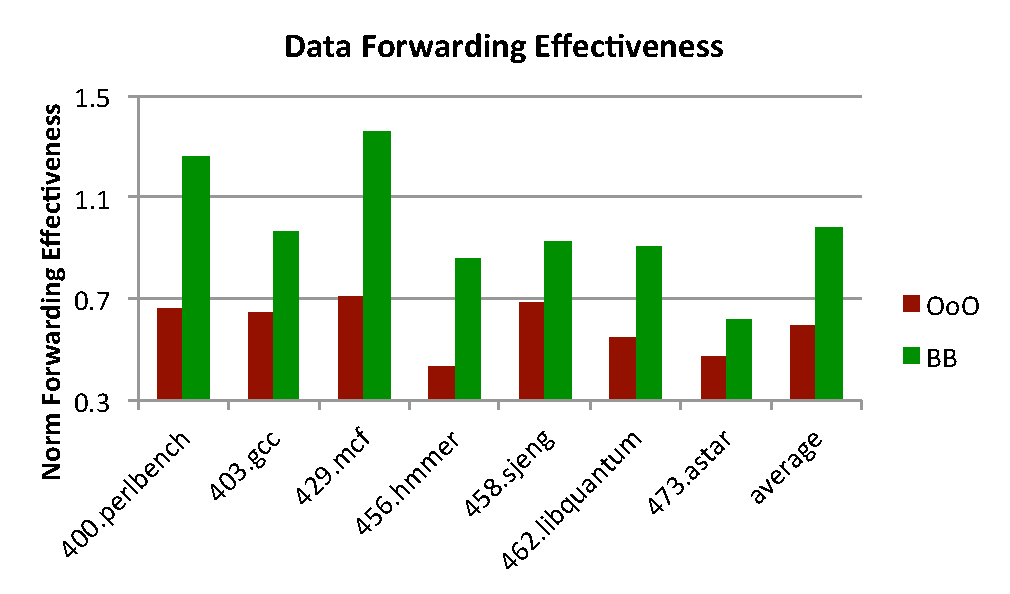
\includegraphics[width=1.0\columnwidth]{result/forwarding.pdf} 
    \caption{Energy vs. Performance Trend for OoO, BB, \& InO}
	\label{fig:forwarding}
\end{figure}

As mentioned in Section~\ref{sec:bpu}, the BB core reduces the number branch
lookup accesses to the branch prediction unit, including the BTB.
Figure~\ref{fig:bpu} illustrates, on average, BB looks up the BPU 35\% less
frequently, making it just as much more energy efficient than OoO.
\begin{figure}[!htbp]
	\centering
	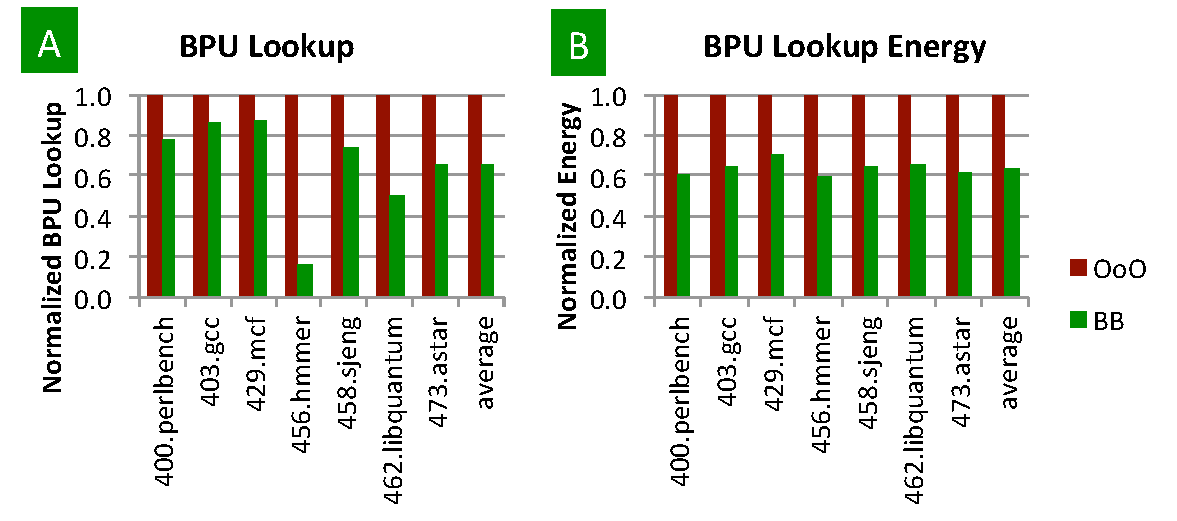
\includegraphics[width=1.0\columnwidth]{result/bpu.pdf} 
    \caption{(A) Normalized ratio of BPU accesses by BBE wrt. OoO. (B)
        Normalized lookup energy reduction ratio of BB wrt. OoO.}
	\label{fig:bpu}
\end{figure}


area evaluation.

energy breakdown pie chart

%evaluation of pipeline stages.
%comparison of new and conventional register rename model.
%comparison of new and conventional squash mode.
%sweep of register file sizes. 



\section{Conclusion}
\label{sec:conclusion}

In this paper presented the basic-block execution model to evaluate the positive
impact of coarse grain out-of-order execution on energy efficiency and
performance. BBE closes 70\% of the performance gap between InO and OoO while
closing 66\% of the energy gap. The performance and energy benefits of BB are
attributed to its effective BPU lookup model, efficient squash model, use BB
window, explicit data forwarding, and the use of local register files.

%\section{outline}
\label{sec:outline}

In this paper I would like to point out the following achievements we have
made:

\begin{itemize} 
    \item energy efficient and high performance computing need for dynamism and
speculation (INTRO)
    \item compiler design
    \item architecture design
    \item pipeline energy efficiency opportunities
    \item ?
    \item results
    \item recovery time, energy, performance, register file behavior, LSQ,
wakeup logic information, having multiple issue elements from each BB
    \item simulation framework
    \item discussion
\end{itemize}


%%%%%%% CITATIONS %%%%%%%
\clearpage
\bstctlcite{bstctl:etal, bstctl:nodash, bstctl:simpurl}
\bibliographystyle{IEEEtranS}
\bibliography{references}

\end{document}

